\documentclass[tikz,border=10pt]{standalone}

\usepackage{xcolor}
\usetikzlibrary{
    arrows.meta,
    positioning,
    fit,
    backgrounds,
    shapes.geometric
}

\begin{document}

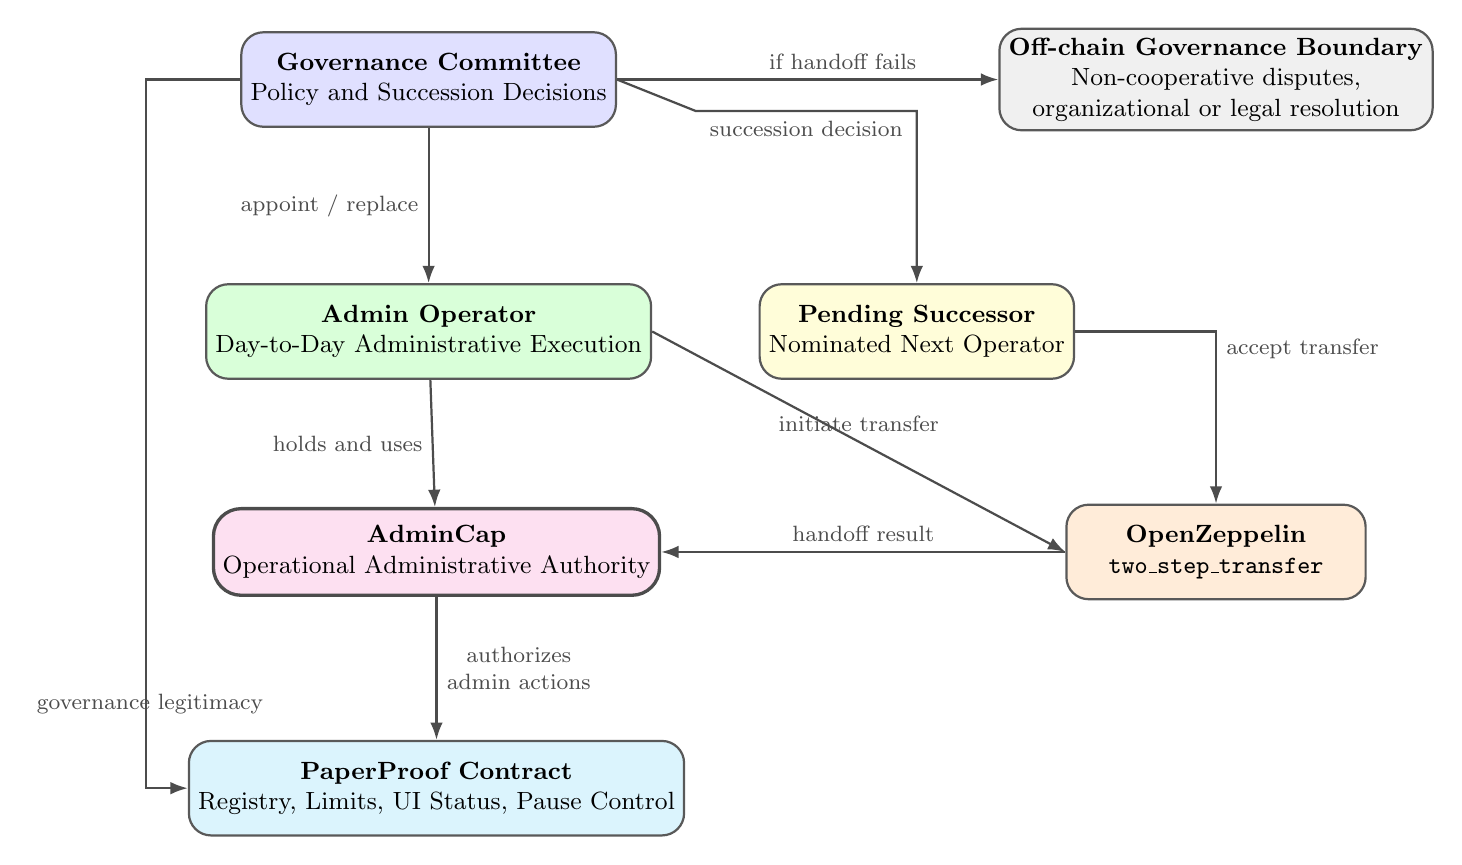
\begin{tikzpicture}[
    font=\small,
    box/.style={
        rectangle,
        rounded corners=8pt,
        draw=black!65,
        thick,
        align=center,
        minimum width=3.8cm,
        minimum height=1.2cm,
        fill=white
    },
    statebox/.style={
        rectangle,
        rounded corners=10pt,
        draw=black!70,
        very thick,
        align=center,
        minimum width=4.0cm,
        minimum height=1.1cm,
        fill=white
    },
    arrow/.style={
        -{Latex[length=2.2mm,width=1.6mm]},
        thick,
        draw=black!70
    },
    note/.style={
        font=\footnotesize,
        align=center,
        text=black!70
    }
]

% =========================================================
% Main governance actors
% =========================================================
\node[box, fill=blue!12] (committee) at (0,0)
{\textbf{Governance Committee}\\Policy and Succession Decisions};

\node[box, fill=green!15] (operator) at (0,-3.2)
{\textbf{Admin Operator}\\Day-to-Day Administrative Execution};

\node[box, fill=yellow!15] (successor) at (6.2,-3.2)
{\textbf{Pending Successor}\\Nominated Next Operator};

% =========================================================
% Capability and contract
% =========================================================
\node[statebox, fill=magenta!12] (admincap) at (0.1,-6.0)
{\textbf{AdminCap}\\Operational Administrative Authority};

\node[box, fill=cyan!14] (contract) at (0.1,-9.0)
{\textbf{PaperProof Contract}\\Registry, Limits, UI Status, Pause Control};

% =========================================================
% OpenZeppelin layer
% =========================================================
\node[box, fill=orange!15] (oz) at (10.0,-6.0)
{\textbf{OpenZeppelin}\\\texttt{two\_step\_transfer}};

% =========================================================
% Off-chain boundary
% =========================================================
\node[box, fill=gray!12] (offchain) at (10.0, 0.0)
{\textbf{Off-chain Governance Boundary}\\Non-cooperative disputes,\\organizational or legal resolution};

% =========================================================
% Main arrows
% =========================================================
\draw[arrow] (committee) -- node[left, note] {appoint / replace} (operator);
\draw[arrow] (operator) -- node[left, note] {holds and uses} (admincap);
\draw[arrow] (admincap) -- node[right, note] {authorizes\\admin actions} (contract);

\draw[arrow] (committee.east) -- ++(1.0,-0.4) -| node[pos=0.25, below, note] {succession decision} (successor.north);

\draw[arrow] (operator.east) -- node[above, note] {initiate transfer} (oz.west);
\draw[arrow] (successor.east) -| node[pos=0.55, right, note] {accept transfer} (oz.north);

\draw[arrow] (oz.west) -- node[above, note] {handoff result} (admincap.east);

\draw[arrow]
    (committee.west) -- ++(-1.2,0)
    -- ++(0,-9.0)
    |- (contract.west)
    node[pos=0.55, above, yshift=23pt,note] {governance legitimacy};


\draw[arrow] (committee.east) to[out=0,in=180] node[pos=0.6, above, note] {if handoff fails} (offchain.west);



\end{tikzpicture}

\end{document}
